%% Creator: Inkscape 0.91, www.inkscape.org
%% PDF/EPS/PS + LaTeX output extension by Johan Engelen, 2010
%% Accompanies image file 'Vzorkovani.pdf' (pdf, eps, ps)
%%
%% To include the image in your LaTeX document, write
%%   \input{<filename>.pdf_tex}
%%  instead of
%%   \includegraphics{<filename>.pdf}
%% To scale the image, write
%%   \def\svgwidth{<desired width>}
%%   \input{<filename>.pdf_tex}
%%  instead of
%%   \includegraphics[width=<desired width>]{<filename>.pdf}
%%
%% Images with a different path to the parent latex file can
%% be accessed with the `import' package (which may need to be
%% installed) using
%%   \usepackage{import}
%% in the preamble, and then including the image with
%%   \import{<path to file>}{<filename>.pdf_tex}
%% Alternatively, one can specify
%%   \graphicspath{{<path to file>/}}
%%
%% For more information, please see info/svg-inkscape on CTAN:
%%   http://tug.ctan.org/tex-archive/info/svg-inkscape
%%
\begingroup%
  \makeatletter%
  \providecommand\color[2][]{%
    \errmessage{(Inkscape) Color is used for the text in Inkscape, but the package 'color.sty' is not loaded}%
    \renewcommand\color[2][]{}%
  }%
  \providecommand\transparent[1]{%
    \errmessage{(Inkscape) Transparency is used (non-zero) for the text in Inkscape, but the package 'transparent.sty' is not loaded}%
    \renewcommand\transparent[1]{}%
  }%
  \providecommand\rotatebox[2]{#2}%
  \ifx\svgwidth\undefined%
    \setlength{\unitlength}{336bp}%
    \ifx\svgscale\undefined%
      \relax%
    \else%
      \setlength{\unitlength}{\unitlength * \real{\svgscale}}%
    \fi%
  \else%
    \setlength{\unitlength}{\svgwidth}%
  \fi%
  \global\let\svgwidth\undefined%
  \global\let\svgscale\undefined%
  \makeatother%
  \begin{picture}(1,0.3452381)%
    \put(0.62285773,0.06666668){\color[rgb]{0,0,0}\makebox(0,0)[lb]{\smash{}}}%
    \put(0.62142808,0.01916617){\color[rgb]{0,0,0}\makebox(0,0)[lb]{\smash{}}}%
    \put(0.8453578,0.82988094){\color[rgb]{0,0,0}\makebox(0,0)[lb]{\smash{}}}%
    \put(0.39000125,0.82988094){\color[rgb]{0,0,0}\makebox(0,0)[lb]{\smash{}}}%
    \put(1.0328588,0.82988094){\color[rgb]{0,0,0}\makebox(0,0)[lb]{\smash{}}}%
    \put(0.09047619,0.19047619){\color[rgb]{0,0,0}\makebox(0,0)[lb]{\smash{}}}%
    \put(0.16254761,0.1595238){\color[rgb]{0,0,0}\makebox(0,0)[lb]{\smash{\footnotesize $W_v$}}}%
    \put(0.13095238,0.10714286){\color[rgb]{0,0,0}\makebox(0,0)[rb]{\smash{\footnotesize $W_u$}}}%
    \put(0.28095239,0.10952381){\color[rgb]{0,0,0}\makebox(0,0)[b]{\smash{\footnotesize $u$}}}%
    \put(0.13095238,0.28095236){\color[rgb]{0,0,0}\makebox(0,0)[rb]{\smash{\footnotesize $v$}}}%
    \put(0.46428662,0.28095236){\color[rgb]{0,0,0}\makebox(0,0)[rb]{\smash{\footnotesize $v$}}}%
    \put(0.79762014,0.28095236){\color[rgb]{0,0,0}\makebox(0,0)[rb]{\smash{\footnotesize $v$}}}%
    \put(0.61428574,0.10952381){\color[rgb]{0,0,0}\makebox(0,0)[b]{\smash{\footnotesize $u$}}}%
    \put(0.9476193,0.10952381){\color[rgb]{0,0,0}\makebox(0,0)[b]{\smash{\footnotesize $u$}}}%
    \put(0.14285714,0.32380953){\color[rgb]{0,0,0}\makebox(0,0)[b]{\smash{$F(u,v)$}}}%
    \put(0.47618952,0.32380953){\color[rgb]{0,0,0}\makebox(0,0)[b]{\smash{$S(u,v)$}}}%
    \put(0.80952308,0.32380953){\color[rgb]{0,0,0}\makebox(0,0)[b]{\smash{$D(u,v)$}}}%
    \put(0.3095239,0.32380953){\color[rgb]{0,0,0}\makebox(0,0)[b]{\smash{$\ast$}}}%
    \put(0.64285642,0.32380953){\color[rgb]{0,0,0}\makebox(0,0)[b]{\smash{$=$}}}%
    \put(0.10714286,0.1547619){\color[rgb]{0,0,0}\makebox(0,0)[rb]{\smash{\footnotesize supp$F$}}}%
    \put(0,0){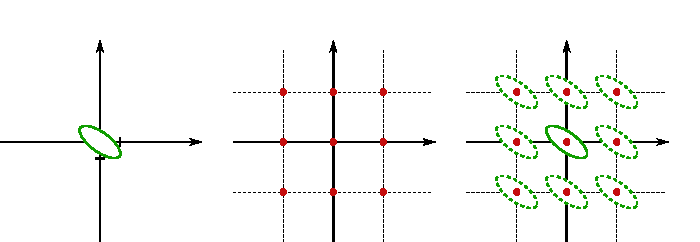
\includegraphics[width=\unitlength,page=1]{Vzorkovani.pdf}}%
  \end{picture}%
\endgroup%
